\documentclass[1p]{elsarticle_modified}
%\bibliographystyle{elsarticle-num}

%\usepackage[colorlinks]{hyperref}
%\usepackage{abbrmath_seonhwa} %\Abb, \Ascr, \Acal ,\Abf, \Afrak
\usepackage{amsfonts}
\usepackage{amssymb}
\usepackage{amsmath}
\usepackage{amsthm}
\usepackage{scalefnt}
\usepackage{amsbsy}
\usepackage{kotex}
\usepackage{caption}
\usepackage{subfig}
\usepackage{color}
\usepackage{graphicx}
\usepackage{xcolor} %% white, black, red, green, blue, cyan, magenta, yellow
\usepackage{float}
\usepackage{setspace}
\usepackage{hyperref}

\usepackage{tikz}
\usetikzlibrary{arrows}

\usepackage{multirow}
\usepackage{array} % fixed length table
\usepackage{hhline}

%%%%%%%%%%%%%%%%%%%%%
\makeatletter
\renewcommand*\env@matrix[1][\arraystretch]{%
	\edef\arraystretch{#1}%
	\hskip -\arraycolsep
	\let\@ifnextchar\new@ifnextchar
	\array{*\c@MaxMatrixCols c}}
\makeatother %https://tex.stackexchange.com/questions/14071/how-can-i-increase-the-line-spacing-in-a-matrix
%%%%%%%%%%%%%%%

\usepackage[normalem]{ulem}

\newcommand{\msout}[1]{\ifmmode\text{\sout{\ensuremath{#1}}}\else\sout{#1}\fi}
%SOURCE: \msout is \stkout macro in https://tex.stackexchange.com/questions/20609/strikeout-in-math-mode

\newcommand{\cancel}[1]{
	\ifmmode
	{\color{red}\msout{#1}}
	\else
	{\color{red}\sout{#1}}
	\fi
}

\newcommand{\add}[1]{
	{\color{blue}\uwave{#1}}
}

\newcommand{\replace}[2]{
	\ifmmode
	{\color{red}\msout{#1}}{\color{blue}\uwave{#2}}
	\else
	{\color{red}\sout{#1}}{\color{blue}\uwave{#2}}
	\fi
}

\newcommand{\Sol}{\mathcal{S}} %segment
\newcommand{\D}{D} %diagram
\newcommand{\A}{\mathcal{A}} %arc


%%%%%%%%%%%%%%%%%%%%%%%%%%%%%5 test

\def\sl{\operatorname{\textup{SL}}(2,\Cbb)}
\def\psl{\operatorname{\textup{PSL}}(2,\Cbb)}
\def\quan{\mkern 1mu \triangleright \mkern 1mu}

\theoremstyle{definition}
\newtheorem{thm}{Theorem}[section]
\newtheorem{prop}[thm]{Proposition}
\newtheorem{lem}[thm]{Lemma}
\newtheorem{ques}[thm]{Question}
\newtheorem{cor}[thm]{Corollary}
\newtheorem{defn}[thm]{Definition}
\newtheorem{exam}[thm]{Example}
\newtheorem{rmk}[thm]{Remark}
\newtheorem{alg}[thm]{Algorithm}

\newcommand{\I}{\sqrt{-1}}
\begin{document}

%\begin{frontmatter}
%
%\title{Boundary parabolic representations of knots up to 8 crossings}
%
%%% Group authors per affiliation:
%\author{Yunhi Cho} 
%\address{Department of Mathematics, University of Seoul, Seoul, Korea}
%\ead{yhcho@uos.ac.kr}
%
%
%\author{Seonhwa Kim} %\fnref{s_kim}}
%\address{Center for Geometry and Physics, Institute for Basic Science, Pohang, 37673, Korea}
%\ead{ryeona17@ibs.re.kr}
%
%\author{Hyuk Kim}
%\address{Department of Mathematical Sciences, Seoul National University, Seoul 08826, Korea}
%\ead{hyukkim@snu.ac.kr}
%
%\author{Seokbeom Yoon}
%\address{Department of Mathematical Sciences, Seoul National University, Seoul, 08826,  Korea}
%\ead{sbyoon15@snu.ac.kr}
%
%\begin{abstract}
%We find all boundary parabolic representation of knots up to 8 crossings.
%
%\end{abstract}
%\begin{keyword}
%    \MSC[2010] 57M25 
%\end{keyword}
%
%\end{frontmatter}

%\linenumbers
%\tableofcontents
%
\newcommand\colored[1]{\textcolor{white}{\rule[-0.35ex]{0.8em}{1.4ex}}\kern-0.8em\color{red} #1}%
%\newcommand\colored[1]{\textcolor{white}{ #1}\kern-2.17ex	\textcolor{white}{ #1}\kern-1.81ex	\textcolor{white}{ #1}\kern-2.15ex\color{red}#1	}

{\Large $\underline{12n_{0399}~(K12n_{0399})}$}

\setlength{\tabcolsep}{10pt}
\renewcommand{\arraystretch}{1.6}
\vspace{1cm}\begin{tabular}{m{100pt}>{\centering\arraybackslash}m{274pt}}
\multirow{5}{120pt}{
	\centering
	\includegraphics[width=112pt]{../../../GIT/diagram.site/Diagrams/png/2488_12n_0399.png}\\
\ \ \ A knot diagram\footnotemark}&
\allowdisplaybreaks
\textbf{Linearized knot diagam} \\
\cline{2-2}
 &
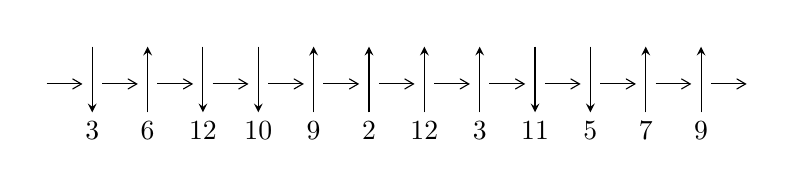
\begin{tikzpicture}[x=20pt, y=17pt]
	% nodes
	\node (C0) at (0, 0) {};
	\node (C1) at (1, 0) {};
	\node (C1U) at (1, +1) {};
	\node (C1D) at (1, -1) {3};

	\node (C2) at (2, 0) {};
	\node (C2U) at (2, +1) {};
	\node (C2D) at (2, -1) {6};

	\node (C3) at (3, 0) {};
	\node (C3U) at (3, +1) {};
	\node (C3D) at (3, -1) {12};

	\node (C4) at (4, 0) {};
	\node (C4U) at (4, +1) {};
	\node (C4D) at (4, -1) {10};

	\node (C5) at (5, 0) {};
	\node (C5U) at (5, +1) {};
	\node (C5D) at (5, -1) {9};

	\node (C6) at (6, 0) {};
	\node (C6U) at (6, +1) {};
	\node (C6D) at (6, -1) {2};

	\node (C7) at (7, 0) {};
	\node (C7U) at (7, +1) {};
	\node (C7D) at (7, -1) {12};

	\node (C8) at (8, 0) {};
	\node (C8U) at (8, +1) {};
	\node (C8D) at (8, -1) {3};

	\node (C9) at (9, 0) {};
	\node (C9U) at (9, +1) {};
	\node (C9D) at (9, -1) {11};

	\node (C10) at (10, 0) {};
	\node (C10U) at (10, +1) {};
	\node (C10D) at (10, -1) {5};

	\node (C11) at (11, 0) {};
	\node (C11U) at (11, +1) {};
	\node (C11D) at (11, -1) {7};

	\node (C12) at (12, 0) {};
	\node (C12U) at (12, +1) {};
	\node (C12D) at (12, -1) {9};
	\node (C13) at (13, 0) {};

	% arrows
	\draw[->,>={angle 60}]
	(C0) edge (C1) (C1) edge (C2) (C2) edge (C3) (C3) edge (C4) (C4) edge (C5) (C5) edge (C6) (C6) edge (C7) (C7) edge (C8) (C8) edge (C9) (C9) edge (C10) (C10) edge (C11) (C11) edge (C12) (C12) edge (C13) ;	\draw[->,>=stealth]
	(C1U) edge (C1D) (C2D) edge (C2U) (C3U) edge (C3D) (C4U) edge (C4D) (C5D) edge (C5U) (C6D) edge (C6U) (C7D) edge (C7U) (C8D) edge (C8U) (C9U) edge (C9D) (C10U) edge (C10D) (C11D) edge (C11U) (C12D) edge (C12U) ;
	\end{tikzpicture} \\
\hhline{~~} \\& 
\textbf{Solving Sequence} \\ \cline{2-2} 
 &
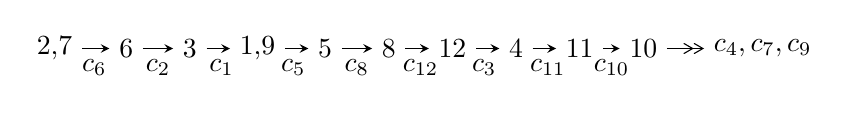
\begin{tikzpicture}[x=23pt, y=7pt]
	% node
	\node (A0) at (-1/8, 0) {2,7};
	\node (A1) at (1, 0) {6};
	\node (A2) at (2, 0) {3};
	\node (A3) at (49/16, 0) {1,9};
	\node (A4) at (33/8, 0) {5};
	\node (A5) at (41/8, 0) {8};
	\node (A6) at (49/8, 0) {12};
	\node (A7) at (57/8, 0) {4};
	\node (A8) at (65/8, 0) {11};
	\node (A9) at (73/8, 0) {10};
	\node (C1) at (1/2, -1) {$c_{6}$};
	\node (C2) at (3/2, -1) {$c_{2}$};
	\node (C3) at (5/2, -1) {$c_{1}$};
	\node (C4) at (29/8, -1) {$c_{5}$};
	\node (C5) at (37/8, -1) {$c_{8}$};
	\node (C6) at (45/8, -1) {$c_{12}$};
	\node (C7) at (53/8, -1) {$c_{3}$};
	\node (C8) at (61/8, -1) {$c_{11}$};
	\node (C9) at (69/8, -1) {$c_{10}$};
	\node (A10) at (11, 0) {$c_{4},c_{7},c_{9}$};

	% edge
	\draw[->,>=stealth]	
	(A0) edge (A1) (A1) edge (A2) (A2) edge (A3) (A3) edge (A4) (A4) edge (A5) (A5) edge (A6) (A6) edge (A7) (A7) edge (A8) (A8) edge (A9) ;
	\draw[->>,>={angle 60}]	
	(A9) edge (A10);
\end{tikzpicture} \\ 

\end{tabular} \\

\footnotetext{
The image of knot diagram is generated by the software ``\textbf{Draw programme}" developed by Andrew Bartholomew(\url{http://www.layer8.co.uk/maths/draw/index.htm\#Running-draw}), where we modified some parts for our purpose(\url{https://github.com/CATsTAILs/LinksPainter}).
}\phantom \\ \newline 
\centering \textbf{Ideals for irreducible components\footnotemark of $X_{\text{par}}$} 
 
\begin{align*}
I^u_{1}&=\langle 
-6.37109\times10^{80} u^{57}-1.84051\times10^{81} u^{56}+\cdots+5.53954\times10^{81} b-2.72456\times10^{81},\\
\phantom{I^u_{1}}&\phantom{= \langle  }1.01217\times10^{81} u^{57}+2.67010\times10^{81} u^{56}+\cdots+5.53954\times10^{81} a+9.31498\times10^{81},\;u^{58}+2 u^{57}+\cdots-27 u+19\rangle \\
I^u_{2}&=\langle 
u^{17}+5 u^{15}+\cdots+b-4,\;- u^{17}- u^{16}+\cdots+a+2,\;u^{18}+u^{17}+\cdots+u+1\rangle \\
\\
\end{align*}
\raggedright * 2 irreducible components of $\dim_{\mathbb{C}}=0$, with total 76 representations.\\
\footnotetext{All coefficients of polynomials are rational numbers. But the coefficients are sometimes approximated in decimal forms when there is not enough margin.}
\newpage
\renewcommand{\arraystretch}{1}
\centering \section*{I. $I^u_{1}= \langle -6.37\times10^{80} u^{57}-1.84\times10^{81} u^{56}+\cdots+5.54\times10^{81} b-2.72\times10^{81},\;1.01\times10^{81} u^{57}+2.67\times10^{81} u^{56}+\cdots+5.54\times10^{81} a+9.31\times10^{81},\;u^{58}+2 u^{57}+\cdots-27 u+19 \rangle$}
\flushleft \textbf{(i) Arc colorings}\\
\begin{tabular}{m{7pt} m{180pt} m{7pt} m{180pt} }
\flushright $a_{2}=$&$\begin{pmatrix}0\\u\end{pmatrix}$ \\
\flushright $a_{7}=$&$\begin{pmatrix}1\\0\end{pmatrix}$ \\
\flushright $a_{6}=$&$\begin{pmatrix}1\\u^2\end{pmatrix}$ \\
\flushright $a_{3}=$&$\begin{pmatrix}u\\u^3+u\end{pmatrix}$ \\
\flushright $a_{1}=$&$\begin{pmatrix}u^3\\u^5+u^3+u\end{pmatrix}$ \\
\flushright $a_{9}=$&$\begin{pmatrix}-0.182717 u^{57}-0.482007 u^{56}+\cdots-0.595250 u-1.68154\\0.115011 u^{57}+0.332249 u^{56}+\cdots-5.79553 u+0.491839\end{pmatrix}$ \\
\flushright $a_{5}=$&$\begin{pmatrix}0.215408 u^{57}+0.599279 u^{56}+\cdots-5.51146 u+2.78906\\0.0682106 u^{57}+0.107706 u^{56}+\cdots+9.01545 u-0.0425585\end{pmatrix}$ \\
\flushright $a_{8}=$&$\begin{pmatrix}-0.0965279 u^{57}-0.205612 u^{56}+\cdots-0.632369 u+0.510681\\0.0864318 u^{57}+0.243238 u^{56}+\cdots-4.66179 u+0.707748\end{pmatrix}$ \\
\flushright $a_{12}=$&$\begin{pmatrix}-0.184306 u^{57}-0.235116 u^{56}+\cdots-7.66825 u+2.57745\\-0.0327982 u^{57}+0.0595320 u^{56}+\cdots-3.43943 u+4.22235\end{pmatrix}$ \\
\flushright $a_{4}=$&$\begin{pmatrix}-0.0364741 u^{57}+0.0502724 u^{56}+\cdots+0.960488 u+0.303105\\-0.115380 u^{57}-0.144572 u^{56}+\cdots-4.33270 u+3.07815\end{pmatrix}$ \\
\flushright $a_{11}=$&$\begin{pmatrix}-0.151508 u^{57}-0.294648 u^{56}+\cdots-4.22882 u-1.64490\\-0.0327982 u^{57}+0.0595320 u^{56}+\cdots-3.43943 u+4.22235\end{pmatrix}$ \\
\flushright $a_{10}=$&$\begin{pmatrix}-0.261480 u^{57}-0.760630 u^{56}+\cdots+1.64155 u-3.31612\\0.0235570 u^{57}+0.113579 u^{56}+\cdots-7.62175 u+0.966758\end{pmatrix}$\\&\end{tabular}
\flushleft \textbf{(ii) Obstruction class $= -1$}\\~\\
\flushleft \textbf{(iii) Cusp Shapes $= -0.0203392 u^{57}-0.188722 u^{56}+\cdots-30.5602 u-6.13312$}\\~\\
\newpage\renewcommand{\arraystretch}{1}
\flushleft \textbf{(iv) u-Polynomials at the component}\newline \\
\begin{tabular}{m{50pt}|m{274pt}}
Crossings & \hspace{64pt}u-Polynomials at each crossing \\
\hline $$\begin{aligned}c_{1}\end{aligned}$$&$\begin{aligned}
&u^{58}+40 u^{57}+\cdots-3009 u+361
\end{aligned}$\\
\hline $$\begin{aligned}c_{2},c_{6}\end{aligned}$$&$\begin{aligned}
&u^{58}-2 u^{57}+\cdots+27 u+19
\end{aligned}$\\
\hline $$\begin{aligned}c_{3}\end{aligned}$$&$\begin{aligned}
&u^{58}-6 u^{57}+\cdots+9863 u+10043
\end{aligned}$\\
\hline $$\begin{aligned}c_{4},c_{10}\end{aligned}$$&$\begin{aligned}
&u^{58}- u^{57}+\cdots-6 u+19
\end{aligned}$\\
\hline $$\begin{aligned}c_{5}\end{aligned}$$&$\begin{aligned}
&u^{58}+30 u^{56}+\cdots-6099 u+2888
\end{aligned}$\\
\hline $$\begin{aligned}c_{7},c_{11}\end{aligned}$$&$\begin{aligned}
&u^{58}-3 u^{57}+\cdots+12 u+1
\end{aligned}$\\
\hline $$\begin{aligned}c_{8}\end{aligned}$$&$\begin{aligned}
&u^{58}- u^{57}+\cdots+958 u+751
\end{aligned}$\\
\hline $$\begin{aligned}c_{9}\end{aligned}$$&$\begin{aligned}
&u^{58}+33 u^{57}+\cdots+3228 u+361
\end{aligned}$\\
\hline $$\begin{aligned}c_{12}\end{aligned}$$&$\begin{aligned}
&u^{58}+3 u^{57}+\cdots+113424 u+119344
\end{aligned}$\\
\hline
\end{tabular}\\~\\
\newpage\renewcommand{\arraystretch}{1}
\flushleft \textbf{(v) Riley Polynomials at the component}\newline \\
\begin{tabular}{m{50pt}|m{274pt}}
Crossings & \hspace{64pt}Riley Polynomials at each crossing \\
\hline $$\begin{aligned}c_{1}\end{aligned}$$&$\begin{aligned}
&y^{58}-32 y^{57}+\cdots-18457409 y+130321
\end{aligned}$\\
\hline $$\begin{aligned}c_{2},c_{6}\end{aligned}$$&$\begin{aligned}
&y^{58}+40 y^{57}+\cdots-3009 y+361
\end{aligned}$\\
\hline $$\begin{aligned}c_{3}\end{aligned}$$&$\begin{aligned}
&y^{58}-72 y^{57}+\cdots-2262348709 y+100861849
\end{aligned}$\\
\hline $$\begin{aligned}c_{4},c_{10}\end{aligned}$$&$\begin{aligned}
&y^{58}-33 y^{57}+\cdots-3228 y+361
\end{aligned}$\\
\hline $$\begin{aligned}c_{5}\end{aligned}$$&$\begin{aligned}
&y^{58}+60 y^{57}+\cdots-6995097 y+8340544
\end{aligned}$\\
\hline $$\begin{aligned}c_{7},c_{11}\end{aligned}$$&$\begin{aligned}
&y^{58}-5 y^{57}+\cdots-26 y+1
\end{aligned}$\\
\hline $$\begin{aligned}c_{8}\end{aligned}$$&$\begin{aligned}
&y^{58}+73 y^{57}+\cdots+20589374 y+564001
\end{aligned}$\\
\hline $$\begin{aligned}c_{9}\end{aligned}$$&$\begin{aligned}
&y^{58}-9 y^{57}+\cdots-449164 y+130321
\end{aligned}$\\
\hline $$\begin{aligned}c_{12}\end{aligned}$$&$\begin{aligned}
&y^{58}+75 y^{57}+\cdots-34418530176 y+14242990336
\end{aligned}$\\
\hline
\end{tabular}\\~\\
\newpage\flushleft \textbf{(vi) Complex Volumes and Cusp Shapes}
$$\begin{array}{c|c|c}  
\text{Solutions to }I^u_{1}& \I (\text{vol} + \sqrt{-1}CS) & \text{Cusp shape}\\
 \hline 
\begin{aligned}
u &= \phantom{-}0.224515 + 1.006340 I \\
a &= -0.33066 - 2.04253 I \\
b &= -0.249830 + 0.006141 I\end{aligned}
 & -2.43095 + 5.91497 I & \phantom{-}2.38973 - 6.67697 I \\ \hline\begin{aligned}
u &= \phantom{-}0.224515 - 1.006340 I \\
a &= -0.33066 + 2.04253 I \\
b &= -0.249830 - 0.006141 I\end{aligned}
 & -2.43095 - 5.91497 I & \phantom{-}2.38973 + 6.67697 I \\ \hline\begin{aligned}
u &= -0.030766 + 0.962352 I \\
a &= -0.06436 + 1.97929 I \\
b &= -0.746000 - 0.276999 I\end{aligned}
 & \phantom{-}0.1036930 + 0.0767330 I & \phantom{-}2.65103 - 0.60139 I \\ \hline\begin{aligned}
u &= -0.030766 - 0.962352 I \\
a &= -0.06436 - 1.97929 I \\
b &= -0.746000 + 0.276999 I\end{aligned}
 & \phantom{-}0.1036930 - 0.0767330 I & \phantom{-}2.65103 + 0.60139 I \\ \hline\begin{aligned}
u &= \phantom{-}1.042920 + 0.032836 I \\
a &= \phantom{-}0.259112 + 0.104770 I \\
b &= \phantom{-}0.68966 - 1.30617 I\end{aligned}
 & -5.37599 - 3.80435 I & \phantom{-}2.65869 + 2.19609 I \\ \hline\begin{aligned}
u &= \phantom{-}1.042920 - 0.032836 I \\
a &= \phantom{-}0.259112 - 0.104770 I \\
b &= \phantom{-}0.68966 + 1.30617 I\end{aligned}
 & -5.37599 + 3.80435 I & \phantom{-}2.65869 - 2.19609 I \\ \hline\begin{aligned}
u &= -1.058870 + 0.161540 I \\
a &= -0.227004 + 0.100851 I \\
b &= -0.095391 - 1.169420 I\end{aligned}
 & -9.58690 + 0.42947 I & -1.63258 - 0.54397 I \\ \hline\begin{aligned}
u &= -1.058870 - 0.161540 I \\
a &= -0.227004 - 0.100851 I \\
b &= -0.095391 + 1.169420 I\end{aligned}
 & -9.58690 - 0.42947 I & -1.63258 + 0.54397 I \\ \hline\begin{aligned}
u &= -0.460132 + 0.780804 I \\
a &= \phantom{-}1.310830 + 0.501042 I \\
b &= \phantom{-}0.519539 - 0.203889 I\end{aligned}
 & \phantom{-}0.07479 - 1.89327 I & \phantom{-}0.15136 + 5.96513 I \\ \hline\begin{aligned}
u &= -0.460132 - 0.780804 I \\
a &= \phantom{-}1.310830 - 0.501042 I \\
b &= \phantom{-}0.519539 + 0.203889 I\end{aligned}
 & \phantom{-}0.07479 + 1.89327 I & \phantom{-}0.15136 - 5.96513 I\\
 \hline 
 \end{array}$$\newpage$$\begin{array}{c|c|c}  
\text{Solutions to }I^u_{1}& \I (\text{vol} + \sqrt{-1}CS) & \text{Cusp shape}\\
 \hline 
\begin{aligned}
u &= \phantom{-}0.105990 + 1.102970 I \\
a &= -0.810233 + 0.184658 I \\
b &= \phantom{-}1.80171 - 0.04967 I\end{aligned}
 & -6.41348 + 2.03025 I & -3.15648 - 3.60193 I \\ \hline\begin{aligned}
u &= \phantom{-}0.105990 - 1.102970 I \\
a &= -0.810233 - 0.184658 I \\
b &= \phantom{-}1.80171 + 0.04967 I\end{aligned}
 & -6.41348 - 2.03025 I & -3.15648 + 3.60193 I \\ \hline\begin{aligned}
u &= \phantom{-}0.561429 + 0.692143 I \\
a &= -0.524254 + 0.648250 I \\
b &= -1.135660 - 0.415124 I\end{aligned}
 & \phantom{-}2.43289 + 1.05533 I & \phantom{-}3.94947 + 2.91901 I \\ \hline\begin{aligned}
u &= \phantom{-}0.561429 - 0.692143 I \\
a &= -0.524254 - 0.648250 I \\
b &= -1.135660 + 0.415124 I\end{aligned}
 & \phantom{-}2.43289 - 1.05533 I & \phantom{-}3.94947 - 2.91901 I \\ \hline\begin{aligned}
u &= -0.761038 + 0.814758 I \\
a &= -0.300716 + 0.114866 I \\
b &= -0.379098 + 0.825252 I\end{aligned}
 & \phantom{-}1.83532 - 4.45936 I & \phantom{-}2.00000 + 6.82517 I \\ \hline\begin{aligned}
u &= -0.761038 - 0.814758 I \\
a &= -0.300716 - 0.114866 I \\
b &= -0.379098 - 0.825252 I\end{aligned}
 & \phantom{-}1.83532 + 4.45936 I & \phantom{-}2.00000 - 6.82517 I \\ \hline\begin{aligned}
u &= -0.319860 + 0.802100 I \\
a &= \phantom{-}1.121730 - 0.655570 I \\
b &= \phantom{-}0.060021 - 0.162688 I\end{aligned}
 & -0.29143 - 1.82126 I & \phantom{-}1.27978 + 4.93251 I \\ \hline\begin{aligned}
u &= -0.319860 - 0.802100 I \\
a &= \phantom{-}1.121730 + 0.655570 I \\
b &= \phantom{-}0.060021 + 0.162688 I\end{aligned}
 & -0.29143 + 1.82126 I & \phantom{-}1.27978 - 4.93251 I \\ \hline\begin{aligned}
u &= -1.172040 + 0.071525 I \\
a &= \phantom{-}0.303741 + 0.232489 I \\
b &= \phantom{-}0.85630 + 1.92853 I\end{aligned}
 & -8.63085 + 8.82241 I & \phantom{-0.000000 } 0. - 5.23324 I \\ \hline\begin{aligned}
u &= -1.172040 - 0.071525 I \\
a &= \phantom{-}0.303741 - 0.232489 I \\
b &= \phantom{-}0.85630 - 1.92853 I\end{aligned}
 & -8.63085 - 8.82241 I & \phantom{-0.000000 -}0. + 5.23324 I\\
 \hline 
 \end{array}$$\newpage$$\begin{array}{c|c|c}  
\text{Solutions to }I^u_{1}& \I (\text{vol} + \sqrt{-1}CS) & \text{Cusp shape}\\
 \hline 
\begin{aligned}
u &= \phantom{-}0.445581 + 1.103690 I \\
a &= \phantom{-}0.70109 - 1.44721 I \\
b &= \phantom{-}0.848763 + 0.587413 I\end{aligned}
 & -4.43655 + 6.03980 I & \phantom{-0.000000 } 0 \\ \hline\begin{aligned}
u &= \phantom{-}0.445581 - 1.103690 I \\
a &= \phantom{-}0.70109 + 1.44721 I \\
b &= \phantom{-}0.848763 - 0.587413 I\end{aligned}
 & -4.43655 - 6.03980 I & \phantom{-0.000000 } 0 \\ \hline\begin{aligned}
u &= -0.260261 + 1.162950 I \\
a &= \phantom{-}0.04311 - 1.85420 I \\
b &= -0.45658 + 1.34791 I\end{aligned}
 & -2.05268 - 3.33538 I & \phantom{-0.000000 } 0 \\ \hline\begin{aligned}
u &= -0.260261 - 1.162950 I \\
a &= \phantom{-}0.04311 + 1.85420 I \\
b &= -0.45658 - 1.34791 I\end{aligned}
 & -2.05268 + 3.33538 I & \phantom{-0.000000 } 0 \\ \hline\begin{aligned}
u &= -0.779441 + 0.907575 I \\
a &= \phantom{-}0.834365 - 0.262759 I \\
b &= -0.075515 - 0.925892 I\end{aligned}
 & \phantom{-}1.58419 - 1.34680 I & \phantom{-0.000000 } 0 \\ \hline\begin{aligned}
u &= -0.779441 - 0.907575 I \\
a &= \phantom{-}0.834365 + 0.262759 I \\
b &= -0.075515 + 0.925892 I\end{aligned}
 & \phantom{-}1.58419 + 1.34680 I & \phantom{-0.000000 } 0 \\ \hline\begin{aligned}
u &= -0.058218 + 1.207240 I \\
a &= \phantom{-}0.39450 - 1.84866 I \\
b &= -1.02773 + 1.06905 I\end{aligned}
 & -4.57241 - 4.54424 I & \phantom{-0.000000 } 0 \\ \hline\begin{aligned}
u &= -0.058218 - 1.207240 I \\
a &= \phantom{-}0.39450 + 1.84866 I \\
b &= -1.02773 - 1.06905 I\end{aligned}
 & -4.57241 + 4.54424 I & \phantom{-0.000000 } 0 \\ \hline\begin{aligned}
u &= \phantom{-}0.094987 + 1.212170 I \\
a &= -0.79398 + 1.46987 I \\
b &= \phantom{-}0.90589 - 1.47169 I\end{aligned}
 & -6.32920 + 0.20167 I & \phantom{-0.000000 } 0 \\ \hline\begin{aligned}
u &= \phantom{-}0.094987 - 1.212170 I \\
a &= -0.79398 - 1.46987 I \\
b &= \phantom{-}0.90589 + 1.47169 I\end{aligned}
 & -6.32920 - 0.20167 I & \phantom{-0.000000 } 0\\
 \hline 
 \end{array}$$\newpage$$\begin{array}{c|c|c}  
\text{Solutions to }I^u_{1}& \I (\text{vol} + \sqrt{-1}CS) & \text{Cusp shape}\\
 \hline 
\begin{aligned}
u &= \phantom{-}0.285200 + 0.724064 I \\
a &= -1.77053 - 0.53984 I \\
b &= \phantom{-}0.832820 - 0.313787 I\end{aligned}
 & -5.14004 - 0.53773 I & -4.31053 - 1.96229 I \\ \hline\begin{aligned}
u &= \phantom{-}0.285200 - 0.724064 I \\
a &= -1.77053 + 0.53984 I \\
b &= \phantom{-}0.832820 + 0.313787 I\end{aligned}
 & -5.14004 + 0.53773 I & -4.31053 + 1.96229 I \\ \hline\begin{aligned}
u &= \phantom{-}0.675255 + 1.080190 I \\
a &= \phantom{-}0.729932 + 0.807985 I \\
b &= -1.32166 + 0.86386 I\end{aligned}
 & \phantom{-}1.20589 + 3.92566 I & \phantom{-0.000000 } 0 \\ \hline\begin{aligned}
u &= \phantom{-}0.675255 - 1.080190 I \\
a &= \phantom{-}0.729932 - 0.807985 I \\
b &= -1.32166 - 0.86386 I\end{aligned}
 & \phantom{-}1.20589 - 3.92566 I & \phantom{-0.000000 } 0 \\ \hline\begin{aligned}
u &= \phantom{-}0.289778 + 1.251810 I \\
a &= -0.14194 + 2.38715 I \\
b &= -0.83641 - 2.21441 I\end{aligned}
 & -4.57902 + 8.23825 I & \phantom{-0.000000 } 0 \\ \hline\begin{aligned}
u &= \phantom{-}0.289778 - 1.251810 I \\
a &= -0.14194 - 2.38715 I \\
b &= -0.83641 + 2.21441 I\end{aligned}
 & -4.57902 - 8.23825 I & \phantom{-0.000000 } 0 \\ \hline\begin{aligned}
u &= \phantom{-}0.502231 + 0.501611 I \\
a &= \phantom{-}1.90990 + 0.84716 I \\
b &= \phantom{-}0.772295 + 0.298643 I\end{aligned}
 & -1.23139 - 2.94700 I & \phantom{-}3.45016 + 2.06974 I \\ \hline\begin{aligned}
u &= \phantom{-}0.502231 - 0.501611 I \\
a &= \phantom{-}1.90990 - 0.84716 I \\
b &= \phantom{-}0.772295 - 0.298643 I\end{aligned}
 & -1.23139 + 2.94700 I & \phantom{-}3.45016 - 2.06974 I \\ \hline\begin{aligned}
u &= \phantom{-}0.614872 + 0.246619 I \\
a &= \phantom{-}0.986845 - 0.142152 I \\
b &= \phantom{-}0.655283 - 0.683736 I\end{aligned}
 & -1.98798 - 1.92106 I & \phantom{-}0.449585 + 0.437051 I \\ \hline\begin{aligned}
u &= \phantom{-}0.614872 - 0.246619 I \\
a &= \phantom{-}0.986845 + 0.142152 I \\
b &= \phantom{-}0.655283 + 0.683736 I\end{aligned}
 & -1.98798 + 1.92106 I & \phantom{-}0.449585 - 0.437051 I\\
 \hline 
 \end{array}$$\newpage$$\begin{array}{c|c|c}  
\text{Solutions to }I^u_{1}& \I (\text{vol} + \sqrt{-1}CS) & \text{Cusp shape}\\
 \hline 
\begin{aligned}
u &= \phantom{-}0.49464 + 1.35074 I \\
a &= -0.934249 + 1.006260 I \\
b &= \phantom{-}0.33871 - 1.44275 I\end{aligned}
 & -9.72891 + 1.63245 I & \phantom{-0.000000 } 0 \\ \hline\begin{aligned}
u &= \phantom{-}0.49464 - 1.35074 I \\
a &= -0.934249 - 1.006260 I \\
b &= \phantom{-}0.33871 + 1.44275 I\end{aligned}
 & -9.72891 - 1.63245 I & \phantom{-0.000000 } 0 \\ \hline\begin{aligned}
u &= \phantom{-}0.53075 + 1.33985 I \\
a &= \phantom{-}0.49560 - 1.71753 I \\
b &= \phantom{-}0.97811 + 1.43333 I\end{aligned}
 & -9.45215 + 9.41732 I & \phantom{-0.000000 } 0 \\ \hline\begin{aligned}
u &= \phantom{-}0.53075 - 1.33985 I \\
a &= \phantom{-}0.49560 + 1.71753 I \\
b &= \phantom{-}0.97811 - 1.43333 I\end{aligned}
 & -9.45215 - 9.41732 I & \phantom{-0.000000 } 0 \\ \hline\begin{aligned}
u &= -0.42609 + 1.38517 I \\
a &= \phantom{-}0.42731 + 1.44092 I \\
b &= \phantom{-}0.22698 - 1.46052 I\end{aligned}
 & -14.5523 - 4.7341 I & \phantom{-0.000000 } 0 \\ \hline\begin{aligned}
u &= -0.42609 - 1.38517 I \\
a &= \phantom{-}0.42731 - 1.44092 I \\
b &= \phantom{-}0.22698 + 1.46052 I\end{aligned}
 & -14.5523 + 4.7341 I & \phantom{-0.000000 } 0 \\ \hline\begin{aligned}
u &= -0.60852 + 1.32238 I \\
a &= -0.779860 - 1.133270 I \\
b &= -0.463346 + 1.215890 I\end{aligned}
 & -13.1569 - 6.4397 I & \phantom{-0.000000 } 0 \\ \hline\begin{aligned}
u &= -0.60852 - 1.32238 I \\
a &= -0.779860 + 1.133270 I \\
b &= -0.463346 - 1.215890 I\end{aligned}
 & -13.1569 + 6.4397 I & \phantom{-0.000000 } 0 \\ \hline\begin{aligned}
u &= \phantom{-}0.07302 + 1.47166 I \\
a &= -1.72282 + 0.30872 I \\
b &= \phantom{-}3.24074 - 0.70291 I\end{aligned}
 & -7.81481 - 1.27231 I & \phantom{-0.000000 } 0 \\ \hline\begin{aligned}
u &= \phantom{-}0.07302 - 1.47166 I \\
a &= -1.72282 - 0.30872 I \\
b &= \phantom{-}3.24074 + 0.70291 I\end{aligned}
 & -7.81481 + 1.27231 I & \phantom{-0.000000 } 0\\
 \hline 
 \end{array}$$\newpage$$\begin{array}{c|c|c}  
\text{Solutions to }I^u_{1}& \I (\text{vol} + \sqrt{-1}CS) & \text{Cusp shape}\\
 \hline 
\begin{aligned}
u &= -0.58987 + 1.38053 I \\
a &= \phantom{-}0.65521 + 1.77053 I \\
b &= \phantom{-}1.32308 - 1.85496 I\end{aligned}
 & -12.7498 - 15.0579 I & \phantom{-0.000000 } 0 \\ \hline\begin{aligned}
u &= -0.58987 - 1.38053 I \\
a &= \phantom{-}0.65521 - 1.77053 I \\
b &= \phantom{-}1.32308 + 1.85496 I\end{aligned}
 & -12.7498 + 15.0579 I & \phantom{-0.000000 } 0 \\ \hline\begin{aligned}
u &= \phantom{-}0.457528 + 0.032139 I \\
a &= \phantom{-}0.782322 - 0.083764 I \\
b &= -0.563932 + 1.221260 I\end{aligned}
 & -0.84917 - 5.20541 I & \phantom{-}3.94046 + 7.52664 I \\ \hline\begin{aligned}
u &= \phantom{-}0.457528 - 0.032139 I \\
a &= \phantom{-}0.782322 + 0.083764 I \\
b &= -0.563932 - 1.221260 I\end{aligned}
 & -0.84917 + 5.20541 I & \phantom{-}3.94046 - 7.52664 I \\ \hline\begin{aligned}
u &= -0.49829 + 1.47862 I \\
a &= -1.10880 - 1.15312 I \\
b &= \phantom{-}0.40920 + 2.41229 I\end{aligned}
 & -13.61300 + 2.78020 I & \phantom{-0.000000 } 0 \\ \hline\begin{aligned}
u &= -0.49829 - 1.47862 I \\
a &= -1.10880 + 1.15312 I \\
b &= \phantom{-}0.40920 - 2.41229 I\end{aligned}
 & -13.61300 - 2.78020 I & \phantom{-0.000000 } 0 \\ \hline\begin{aligned}
u &= -0.375315 + 0.010677 I \\
a &= \phantom{-}0.974844 - 0.096938 I \\
b &= -0.607935 + 0.541636 I\end{aligned}
 & \phantom{-}1.209710 - 0.655189 I & \phantom{-}7.50833 + 2.44087 I \\ \hline\begin{aligned}
u &= -0.375315 - 0.010677 I \\
a &= \phantom{-}0.974844 + 0.096938 I \\
b &= -0.607935 - 0.541636 I\end{aligned}
 & \phantom{-}1.209710 + 0.655189 I & \phantom{-}7.50833 - 2.44087 I\\
 \hline 
 \end{array}$$\newpage\newpage\renewcommand{\arraystretch}{1}
\centering \section*{II. $I^u_{2}= \langle u^{17}+5 u^{15}+\cdots+b-4,\;- u^{17}- u^{16}+\cdots+a+2,\;u^{18}+u^{17}+\cdots+u+1 \rangle$}
\flushleft \textbf{(i) Arc colorings}\\
\begin{tabular}{m{7pt} m{180pt} m{7pt} m{180pt} }
\flushright $a_{2}=$&$\begin{pmatrix}0\\u\end{pmatrix}$ \\
\flushright $a_{7}=$&$\begin{pmatrix}1\\0\end{pmatrix}$ \\
\flushright $a_{6}=$&$\begin{pmatrix}1\\u^2\end{pmatrix}$ \\
\flushright $a_{3}=$&$\begin{pmatrix}u\\u^3+u\end{pmatrix}$ \\
\flushright $a_{1}=$&$\begin{pmatrix}u^3\\u^5+u^3+u\end{pmatrix}$ \\
\flushright $a_{9}=$&$\begin{pmatrix}u^{17}+u^{16}+\cdots+u-2\\- u^{17}-5 u^{15}+\cdots-2 u+4\end{pmatrix}$ \\
\flushright $a_{5}=$&$\begin{pmatrix}-3 u^{17}-4 u^{16}+\cdots- u-6\\-3 u^{17}-2 u^{16}+\cdots-8 u-1\end{pmatrix}$ \\
\flushright $a_{8}=$&$\begin{pmatrix}u^{17}+u^{16}+\cdots+u-1\\- u^{17}-5 u^{15}+\cdots-2 u+5\end{pmatrix}$ \\
\flushright $a_{12}=$&$\begin{pmatrix}- u^{17}-5 u^{16}+\cdots-8 u-5\\u^{17}+u^{16}+\cdots+7 u+1\end{pmatrix}$ \\
\flushright $a_{4}=$&$\begin{pmatrix}4 u^{17}+11 u^{16}+\cdots+20 u+12\\- u^{17}- u^{16}+\cdots-7 u-1\end{pmatrix}$ \\
\flushright $a_{11}=$&$\begin{pmatrix}-2 u^{17}-6 u^{16}+\cdots-15 u-6\\u^{17}+u^{16}+\cdots+7 u+1\end{pmatrix}$ \\
\flushright $a_{10}=$&$\begin{pmatrix}2 u^{17}+3 u^{16}+\cdots-5 u+5\\3 u^{17}+2 u^{16}+\cdots+8 u+2\end{pmatrix}$\\&\end{tabular}
\flushleft \textbf{(ii) Obstruction class $= 1$}\\~\\
\flushleft \textbf{(iii) Cusp Shapes $= 18 u^{17}+20 u^{16}+102 u^{15}+96 u^{14}+289 u^{13}+242 u^{12}+565 u^{11}+422 u^{10}+770 u^9+505 u^8+760 u^7+449 u^6+540 u^5+268 u^4+235 u^3+107 u^2+48 u+17$}\\~\\
\newpage\renewcommand{\arraystretch}{1}
\flushleft \textbf{(iv) u-Polynomials at the component}\newline \\
\begin{tabular}{m{50pt}|m{274pt}}
Crossings & \hspace{64pt}u-Polynomials at each crossing \\
\hline $$\begin{aligned}c_{1}\end{aligned}$$&$\begin{aligned}
&u^{18}-11 u^{17}+\cdots-15 u+1
\end{aligned}$\\
\hline $$\begin{aligned}c_{2}\end{aligned}$$&$\begin{aligned}
&u^{18}- u^{17}+\cdots- u+1
\end{aligned}$\\
\hline $$\begin{aligned}c_{3}\end{aligned}$$&$\begin{aligned}
&u^{18}+7 u^{17}+\cdots+7 u+1
\end{aligned}$\\
\hline $$\begin{aligned}c_{4}\end{aligned}$$&$\begin{aligned}
&u^{18}-5 u^{16}+\cdots-4 u^2+1
\end{aligned}$\\
\hline $$\begin{aligned}c_{5}\end{aligned}$$&$\begin{aligned}
&u^{18}+3 u^{17}+\cdots-2 u^2+1
\end{aligned}$\\
\hline $$\begin{aligned}c_{6}\end{aligned}$$&$\begin{aligned}
&u^{18}+u^{17}+\cdots+u+1
\end{aligned}$\\
\hline $$\begin{aligned}c_{7}\end{aligned}$$&$\begin{aligned}
&u^{18}-2 u^{17}+\cdots-2 u+1
\end{aligned}$\\
\hline $$\begin{aligned}c_{8}\end{aligned}$$&$\begin{aligned}
&u^{18}+10 u^{16}+\cdots+9 u^2+1
\end{aligned}$\\
\hline $$\begin{aligned}c_{9}\end{aligned}$$&$\begin{aligned}
&u^{18}-10 u^{17}+\cdots-8 u+1
\end{aligned}$\\
\hline $$\begin{aligned}c_{10}\end{aligned}$$&$\begin{aligned}
&u^{18}-5 u^{16}+\cdots-4 u^2+1
\end{aligned}$\\
\hline $$\begin{aligned}c_{11}\end{aligned}$$&$\begin{aligned}
&u^{18}+2 u^{17}+\cdots+2 u+1
\end{aligned}$\\
\hline $$\begin{aligned}c_{12}\end{aligned}$$&$\begin{aligned}
&u^{18}+2 u^{17}+\cdots+2 u+1
\end{aligned}$\\
\hline
\end{tabular}\\~\\
\newpage\renewcommand{\arraystretch}{1}
\flushleft \textbf{(v) Riley Polynomials at the component}\newline \\
\begin{tabular}{m{50pt}|m{274pt}}
Crossings & \hspace{64pt}Riley Polynomials at each crossing \\
\hline $$\begin{aligned}c_{1}\end{aligned}$$&$\begin{aligned}
&y^{18}+3 y^{17}+\cdots-21 y+1
\end{aligned}$\\
\hline $$\begin{aligned}c_{2},c_{6}\end{aligned}$$&$\begin{aligned}
&y^{18}+11 y^{17}+\cdots+15 y+1
\end{aligned}$\\
\hline $$\begin{aligned}c_{3}\end{aligned}$$&$\begin{aligned}
&y^{18}- y^{17}+\cdots+7 y+1
\end{aligned}$\\
\hline $$\begin{aligned}c_{4},c_{10}\end{aligned}$$&$\begin{aligned}
&y^{18}-10 y^{17}+\cdots-8 y+1
\end{aligned}$\\
\hline $$\begin{aligned}c_{5}\end{aligned}$$&$\begin{aligned}
&y^{18}+15 y^{17}+\cdots-4 y+1
\end{aligned}$\\
\hline $$\begin{aligned}c_{7},c_{11}\end{aligned}$$&$\begin{aligned}
&y^{18}-10 y^{17}+\cdots-6 y+1
\end{aligned}$\\
\hline $$\begin{aligned}c_{8}\end{aligned}$$&$\begin{aligned}
&y^{18}+20 y^{17}+\cdots+18 y+1
\end{aligned}$\\
\hline $$\begin{aligned}c_{9}\end{aligned}$$&$\begin{aligned}
&y^{18}+2 y^{17}+\cdots+8 y+1
\end{aligned}$\\
\hline $$\begin{aligned}c_{12}\end{aligned}$$&$\begin{aligned}
&y^{18}-6 y^{17}+\cdots-10 y+1
\end{aligned}$\\
\hline
\end{tabular}\\~\\
\newpage\flushleft \textbf{(vi) Complex Volumes and Cusp Shapes}
$$\begin{array}{c|c|c}  
\text{Solutions to }I^u_{2}& \I (\text{vol} + \sqrt{-1}CS) & \text{Cusp shape}\\
 \hline 
\begin{aligned}
u &= \phantom{-}0.663427 + 0.812489 I \\
a &= -0.1067230 + 0.0051625 I \\
b &= -0.687075 - 0.298572 I\end{aligned}
 & \phantom{-}2.56473 + 2.09263 I & \phantom{-}6.27509 - 4.65916 I \\ \hline\begin{aligned}
u &= \phantom{-}0.663427 - 0.812489 I \\
a &= -0.1067230 - 0.0051625 I \\
b &= -0.687075 + 0.298572 I\end{aligned}
 & \phantom{-}2.56473 - 2.09263 I & \phantom{-}6.27509 + 4.65916 I \\ \hline\begin{aligned}
u &= \phantom{-}0.329171 + 0.866966 I \\
a &= -1.23220 + 1.42346 I \\
b &= -0.738933 + 0.005475 I\end{aligned}
 & \phantom{-}0.76853 + 1.42826 I & \phantom{-}8.35176 - 2.38264 I \\ \hline\begin{aligned}
u &= \phantom{-}0.329171 - 0.866966 I \\
a &= -1.23220 - 1.42346 I \\
b &= -0.738933 - 0.005475 I\end{aligned}
 & \phantom{-}0.76853 - 1.42826 I & \phantom{-}8.35176 + 2.38264 I \\ \hline\begin{aligned}
u &= -0.767733 + 0.810239 I \\
a &= \phantom{-}0.224536 + 0.562717 I \\
b &= \phantom{-}0.019830 + 0.688255 I\end{aligned}
 & \phantom{-}0.91380 - 6.14020 I & \phantom{-}1.38743 + 7.79716 I \\ \hline\begin{aligned}
u &= -0.767733 - 0.810239 I \\
a &= \phantom{-}0.224536 - 0.562717 I \\
b &= \phantom{-}0.019830 - 0.688255 I\end{aligned}
 & \phantom{-}0.91380 + 6.14020 I & \phantom{-}1.38743 - 7.79716 I \\ \hline\begin{aligned}
u &= -0.308872 + 1.108840 I \\
a &= -0.40762 - 2.27471 I \\
b &= -0.723271 + 0.879058 I\end{aligned}
 & -3.46207 - 6.59532 I & -0.29237 + 8.93365 I \\ \hline\begin{aligned}
u &= -0.308872 - 1.108840 I \\
a &= -0.40762 + 2.27471 I \\
b &= -0.723271 - 0.879058 I\end{aligned}
 & -3.46207 + 6.59532 I & -0.29237 - 8.93365 I \\ \hline\begin{aligned}
u &= \phantom{-}0.676502 + 0.985205 I \\
a &= \phantom{-}0.784868 + 0.696433 I \\
b &= -0.781651 + 0.705840 I\end{aligned}
 & \phantom{-}2.01899 + 3.08515 I & \phantom{-}4.31503 - 1.55560 I \\ \hline\begin{aligned}
u &= \phantom{-}0.676502 - 0.985205 I \\
a &= \phantom{-}0.784868 - 0.696433 I \\
b &= -0.781651 - 0.705840 I\end{aligned}
 & \phantom{-}2.01899 - 3.08515 I & \phantom{-}4.31503 + 1.55560 I\\
 \hline 
 \end{array}$$\newpage$$\begin{array}{c|c|c}  
\text{Solutions to }I^u_{2}& \I (\text{vol} + \sqrt{-1}CS) & \text{Cusp shape}\\
 \hline 
\begin{aligned}
u &= -0.777605 + 0.946138 I \\
a &= \phantom{-}1.105390 + 0.065108 I \\
b &= \phantom{-}0.299715 - 0.762984 I\end{aligned}
 & \phantom{-}0.504540 + 0.309567 I & -0.80740 - 1.43142 I \\ \hline\begin{aligned}
u &= -0.777605 - 0.946138 I \\
a &= \phantom{-}1.105390 - 0.065108 I \\
b &= \phantom{-}0.299715 + 0.762984 I\end{aligned}
 & \phantom{-}0.504540 - 0.309567 I & -0.80740 + 1.43142 I \\ \hline\begin{aligned}
u &= -0.236516 + 0.684902 I \\
a &= -1.95856 - 0.66471 I \\
b &= -0.452798 - 0.606876 I\end{aligned}
 & -1.79616 + 4.18945 I & -0.25895 - 4.46563 I \\ \hline\begin{aligned}
u &= -0.236516 - 0.684902 I \\
a &= -1.95856 + 0.66471 I \\
b &= -0.452798 + 0.606876 I\end{aligned}
 & -1.79616 - 4.18945 I & -0.25895 + 4.46563 I \\ \hline\begin{aligned}
u &= -0.043389 + 1.388640 I \\
a &= -1.70876 - 0.48185 I \\
b &= \phantom{-}2.96850 + 0.74047 I\end{aligned}
 & -8.29244 + 1.00000 I & -10.45781 + 0.99918 I \\ \hline\begin{aligned}
u &= -0.043389 - 1.388640 I \\
a &= -1.70876 + 0.48185 I \\
b &= \phantom{-}2.96850 - 0.74047 I\end{aligned}
 & -8.29244 - 1.00000 I & -10.45781 - 0.99918 I \\ \hline\begin{aligned}
u &= -0.034984 + 0.541926 I \\
a &= -2.20094 - 0.05979 I \\
b &= \phantom{-}1.095690 - 0.356910 I\end{aligned}
 & -4.73446 - 1.37974 I & \phantom{-}0.98722 + 4.89065 I \\ \hline\begin{aligned}
u &= -0.034984 - 0.541926 I \\
a &= -2.20094 + 0.05979 I \\
b &= \phantom{-}1.095690 + 0.356910 I\end{aligned}
 & -4.73446 + 1.37974 I & \phantom{-}0.98722 - 4.89065 I\\
 \hline 
 \end{array}$$\newpage
\newpage\renewcommand{\arraystretch}{1}
\centering \section*{ III. u-Polynomials}
\begin{tabular}{m{50pt}|m{274pt}}
Crossings & \hspace{64pt}u-Polynomials at each crossing \\
\hline $$\begin{aligned}c_{1}\end{aligned}$$&$\begin{aligned}
&(u^{18}-11 u^{17}+\cdots-15 u+1)(u^{58}+40 u^{57}+\cdots-3009 u+361)
\end{aligned}$\\
\hline $$\begin{aligned}c_{2}\end{aligned}$$&$\begin{aligned}
&(u^{18}- u^{17}+\cdots- u+1)(u^{58}-2 u^{57}+\cdots+27 u+19)
\end{aligned}$\\
\hline $$\begin{aligned}c_{3}\end{aligned}$$&$\begin{aligned}
&(u^{18}+7 u^{17}+\cdots+7 u+1)(u^{58}-6 u^{57}+\cdots+9863 u+10043)
\end{aligned}$\\
\hline $$\begin{aligned}c_{4}\end{aligned}$$&$\begin{aligned}
&(u^{18}-5 u^{16}+\cdots-4 u^2+1)(u^{58}- u^{57}+\cdots-6 u+19)
\end{aligned}$\\
\hline $$\begin{aligned}c_{5}\end{aligned}$$&$\begin{aligned}
&(u^{18}+3 u^{17}+\cdots-2 u^2+1)(u^{58}+30 u^{56}+\cdots-6099 u+2888)
\end{aligned}$\\
\hline $$\begin{aligned}c_{6}\end{aligned}$$&$\begin{aligned}
&(u^{18}+u^{17}+\cdots+u+1)(u^{58}-2 u^{57}+\cdots+27 u+19)
\end{aligned}$\\
\hline $$\begin{aligned}c_{7}\end{aligned}$$&$\begin{aligned}
&(u^{18}-2 u^{17}+\cdots-2 u+1)(u^{58}-3 u^{57}+\cdots+12 u+1)
\end{aligned}$\\
\hline $$\begin{aligned}c_{8}\end{aligned}$$&$\begin{aligned}
&(u^{18}+10 u^{16}+\cdots+9 u^2+1)(u^{58}- u^{57}+\cdots+958 u+751)
\end{aligned}$\\
\hline $$\begin{aligned}c_{9}\end{aligned}$$&$\begin{aligned}
&(u^{18}-10 u^{17}+\cdots-8 u+1)(u^{58}+33 u^{57}+\cdots+3228 u+361)
\end{aligned}$\\
\hline $$\begin{aligned}c_{10}\end{aligned}$$&$\begin{aligned}
&(u^{18}-5 u^{16}+\cdots-4 u^2+1)(u^{58}- u^{57}+\cdots-6 u+19)
\end{aligned}$\\
\hline $$\begin{aligned}c_{11}\end{aligned}$$&$\begin{aligned}
&(u^{18}+2 u^{17}+\cdots+2 u+1)(u^{58}-3 u^{57}+\cdots+12 u+1)
\end{aligned}$\\
\hline $$\begin{aligned}c_{12}\end{aligned}$$&$\begin{aligned}
&(u^{18}+2 u^{17}+\cdots+2 u+1)(u^{58}+3 u^{57}+\cdots+113424 u+119344)
\end{aligned}$\\
\hline
\end{tabular}\newpage\renewcommand{\arraystretch}{1}
\centering \section*{ IV. Riley Polynomials}
\begin{tabular}{m{50pt}|m{274pt}}
Crossings & \hspace{64pt}Riley Polynomials at each crossing \\
\hline $$\begin{aligned}c_{1}\end{aligned}$$&$\begin{aligned}
&(y^{18}+3 y^{17}+\cdots-21 y+1)\\
&\cdot(y^{58}-32 y^{57}+\cdots-18457409 y+130321)
\end{aligned}$\\
\hline $$\begin{aligned}c_{2},c_{6}\end{aligned}$$&$\begin{aligned}
&(y^{18}+11 y^{17}+\cdots+15 y+1)(y^{58}+40 y^{57}+\cdots-3009 y+361)
\end{aligned}$\\
\hline $$\begin{aligned}c_{3}\end{aligned}$$&$\begin{aligned}
&(y^{18}- y^{17}+\cdots+7 y+1)\\
&\cdot(y^{58}-72 y^{57}+\cdots-2262348709 y+100861849)
\end{aligned}$\\
\hline $$\begin{aligned}c_{4},c_{10}\end{aligned}$$&$\begin{aligned}
&(y^{18}-10 y^{17}+\cdots-8 y+1)(y^{58}-33 y^{57}+\cdots-3228 y+361)
\end{aligned}$\\
\hline $$\begin{aligned}c_{5}\end{aligned}$$&$\begin{aligned}
&(y^{18}+15 y^{17}+\cdots-4 y+1)\\
&\cdot(y^{58}+60 y^{57}+\cdots-6995097 y+8340544)
\end{aligned}$\\
\hline $$\begin{aligned}c_{7},c_{11}\end{aligned}$$&$\begin{aligned}
&(y^{18}-10 y^{17}+\cdots-6 y+1)(y^{58}-5 y^{57}+\cdots-26 y+1)
\end{aligned}$\\
\hline $$\begin{aligned}c_{8}\end{aligned}$$&$\begin{aligned}
&(y^{18}+20 y^{17}+\cdots+18 y+1)\\
&\cdot(y^{58}+73 y^{57}+\cdots+20589374 y+564001)
\end{aligned}$\\
\hline $$\begin{aligned}c_{9}\end{aligned}$$&$\begin{aligned}
&(y^{18}+2 y^{17}+\cdots+8 y+1)(y^{58}-9 y^{57}+\cdots-449164 y+130321)
\end{aligned}$\\
\hline $$\begin{aligned}c_{12}\end{aligned}$$&$\begin{aligned}
&(y^{18}-6 y^{17}+\cdots-10 y+1)\\
&\cdot(y^{58}+75 y^{57}+\cdots-34418530176 y+14242990336)
\end{aligned}$\\
\hline
\end{tabular}
\vskip 2pc
\end{document}